\section{Discussion}
\label{sec:discussion}





\subsection{Managing \kvcache via Unified Memory}

To enable dynamic memory allocation, we also considered leveraging unified memory via \cudamallocmanaged~\cite{nvidia-cuda,gpu-mismanaged}. However, we find that unified memory support is currently not suitable for serving LLMs. First, it does not support partial freeing, preventing reclamation of physical memory of individual requests. Second, it lacks support for memory aliasing which prevents de-duplication of \kvcache content in physical memory (de-duplication is useful when requests share a common prefix~\cite{vllmsosp}), consequently limiting batch size. \cudamallocmanaged also allocates 2MB pages by default which can cause severe fragmentation. However, our changes in NVIDIA drivers are based on unified memory: we allocate virtual tensors using \cudamallocmanaged, enabling support for partial freeing and page sharing with additional APIs. In addition, we introduce latency hiding optimizations and support for smaller pages. Therefore, one could consider our extensions to NVIDIA drivers as ``unified memory optimized for LLM serving''.

\begin{table}[t!]
\scalebox{0.9}{
% \color{black}\begin{tabular}{l|rcc}
\color{black}\begin{tabular}{l@{\hspace{6pt}}|c@{\hspace{6pt}}|c@{\hspace{6pt}}} \\
\multirow{2}{*}{\textbf{Model}} & \multicolumn{2}{c}{\textbf{Block size (\# Tokens in a 2MB page)}} \\ 
 &  w/o Tensor Slicing & w/ Tensor Slicing \\ \toprule
\yismall (TP-1) & 2048 & 64  \\
\yismall (TP-2) & 4096 & 128 \\ \hline
\llamasmall (TP-1) & 1024 & 32  \\
\llamasmall (TP-2) & 2048 & 64 \\ \hline
\yimedium (TP-1) & 1024 & 18 \\
\yimedium (TP-2) & 2048 & 36\\  \bottomrule
\end{tabular}}
\caption{\kvcache block size with and without tensor slicing with 2MB pages.}
\label{table:eval:megacache:blocksize}
\end{table}


\subsection{Reducing Fragmentation via Tensor Slicing}
To reduce fragmentation caused by 2MB pages, we also provide an alternative method that does not require modifying  NVIDIA drivers. In this method, we use a single 2MB page to store the \kvcache tokens of all layers for a given request. This can be done by allocating one virtual tensor of shape $[B, L, N, H, D]$ for \kcache (and one for \vcache) and slicing it across all layers, instead of allocating $2\times N$ virtual tensors of shape $[B, L, H, D]$. This reduces fragmentation to $1/N$ of the prior design as shown in~\autoref{table:eval:megacache:blocksize}. In this design, the \kcache (or \vcache) of a particular layer $n$ is represented by slice $[B, L, n:n+1, H, D]$ of the original tensor, and can be passed to attention kernels for computation. However, note that with tensor slicing, the \kcache (and \vcache) of each layer is no longer contiguous. Computing attention over such a tensor slice is possible only if the the attention kernel supports memory addressing with strides. While many kernels (e.g., \flashattention) support strides out-of-the-box, the earlier versions of \flashinfer lacked such support~\cite{fi-strides}. Therefore, relying on tensor slicing as the primary method of reducing fragmentation would have prevented \sysname from supporting \flashinfer kernels. Hence, to support unmodified \flashinfer kernels, we chose to add support for smaller pages in NVIDIA drivers. Importantly, our two solutions are compatible with each other; one could deploy smaller pages with tensor slicing to further reduce fragmentation, if required.


%Given a model with N layers, for every token, if memory for its KV vectors at all layers is allocated for in a contiguously, the block size can be reduced to 1/N of its original size, thus reducing the effect of fragmentation considerably. Thus, the layout of such a K cache / V cache would be  instead of . We refer to this scheme as MegaCache. Table \ref{table:eval:megacache:blocksize} quantifies the reduction in block size for different models from the paper.

%However, the drawback of such an approach is that, the attention kernel accessing it must be enabled with support for stride-d tensor access, which is still non-contiguity in some form. Most kernels do support strides today, but early versions of \flashinfer did not support this, thus necessitating the alternative to enable their use.



\subsection{Programming Effort}
PagedAttention requires significant programming effort. For example, integrating \flashinfer decode kernels in \vllm required  more than 600 lines of code changes in over 15 files~\cite{vllmfi1,vllmfi2,vllmfi3}. Implementing the initial paging support in \flashattention kernel also required $\approx 280$ lines of code changes~\cite{fapaging} and additional efforts to support small block sizes~\cite{fasmall}. In contrast, \sysname makes it feasible to replace one attention kernel with another with only a few lines of code changes in the serving framework (\autoref{fig:eval:codediff}). Note that the example shown in~\autoref{fig:eval:codediff} has no interaction with memory management; this is precisely the goal of \sysname, i.e., when a slow kernel is replaced by a fast kernel, memory management should continue to work transparently.


\begin{figure}[t!]
    \centering
    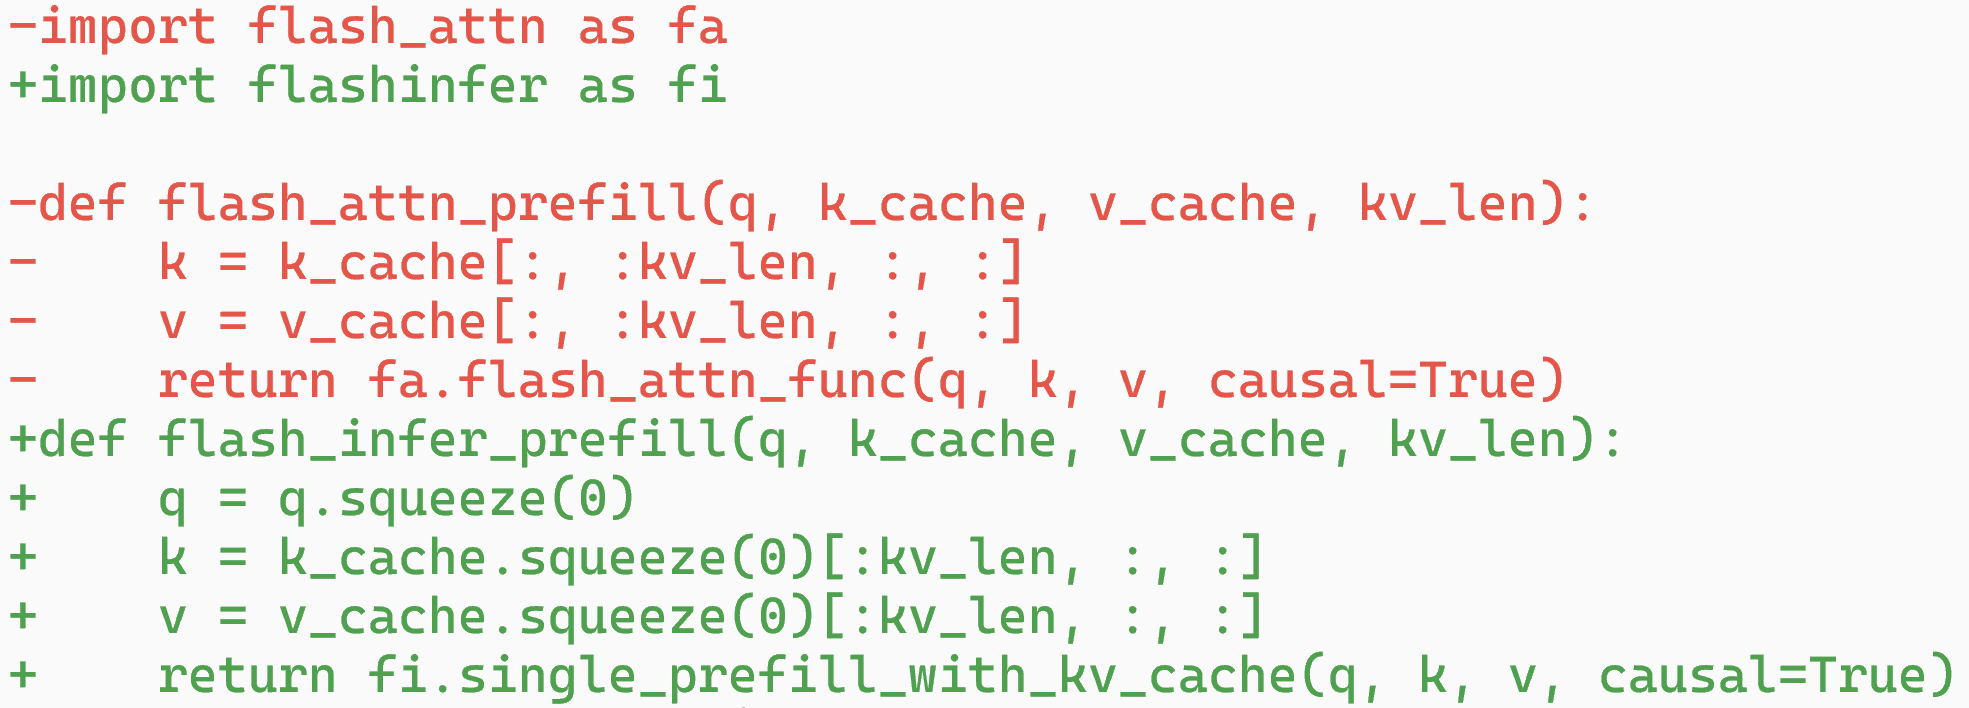
\includegraphics[width=0.85\columnwidth]{figures/fa_fi_code_diff.png}
    \caption{Illustration of code changes needed to replace the prefill attention kernel of \flashattention by \flashinfer when using \sysname for memory allocation.}
    \label{fig:eval:codediff}
\end{figure}

\begin{comment}
\begin{table}[t!]
\scalebox{0.8}{
\begin{tabular}{lcccc}
 & \multirow{2}{*}{\begin{tabular}[c]{@{}c@{}}Batch\\Size\end{tabular}} & \multirow{2}{*}{\begin{tabular}[c]{@{}c@{}}\fapaged\\(Block Size = 256)\end{tabular}} & \multirow{2}{*}{\begin{tabular}[c]{@{}c@{}}\fapaged\\(Block Size = 16)\end{tabular}} & \\ 
Model & & & & Ratio \\ \toprule
\multirow{2}{*}{Yi-6B} & 1 & 0.085 & 0.085 & $1.00\times$ \\
 & 2 & 0.093 & 0.094 & $1.01\times$ \\
 & 4 & 0.109 & 0.115 & $1.05\times$ \\ \hdashline 
\multirow{3}{*}{\begin{tabular}[c]{@{}l@{}}Llama-3\\ -8B\end{tabular}} & 1 & 0.076 & 0.082 & $1.08\times$ \\
 & 2 & 0.097 & 0.105 & $1.07\times$ \\
 & 4 & 0.136 & 0.143 & $1.05\times$ \\ \hdashline
\multirow{3}{*}{Yi-34B} & 1 & 0.070 & 0.076 & $1.09\times$ \\
 & 2 & 0.088 & 0.095 & $1.08\times$ \\
 & 4 & 0.116 & 0.117 & $1.01\times$ \\ \bottomrule
\end{tabular}}
\caption{Impact of varying block size on the execution latency (in milliseconds) of \flashattention decode kernel.}
\label{table:fa:blocksize}
\end{table}

\subsection{Further Analysis of Internal Fragmentation}

\sysname uses page size as the unit of physical memory allocation as opposed to the \pa's unit of \kvcache block size. Therefore, it is natural to ask \textit{what is the relationship between page size and block size}. To compute this relationship, let $S$ be the size of a single token's per-layer K-cache (or V-cache) on a worker (see~\autoref{sec:design:buffersize}). Then, page size t translates to \kvcache block size $= t/S$. Note that $S=H\times D\times P$, where $H$ is the number of KV heads on a worker, $D$ is the dimension of each KV head and $P$ is the number of bytes based on model precision (e.g., P=2 for FP16/BF16). Therefore, block size = $t/(H\times D\times P)$.


\autoref{table:eval:blocksize:fragmentation} shows the block size for different model configurations and physical memory allocation sizes; we show each model under two TP configurations -- TP-1 and TP-2 -- to highlight the effect of TP dimension on block size. In addition, the table also shows how much physical memory can be (theoretically) wasted by \sysname due to internal fragmentation in the worst-case. The worst-case occurs when a new page is allocated but remains completely unused.


\begin{table}[t!]
\scalebox{0.85}{
\begin{tabular}{ccccc}
Context Length & Batch Size & FI\_NonPaged & \fipaged & Ratio \\ \toprule
8K & 4 & 0.902 & 0.071 & $12.7\times$ \\
8K & 8 & 0.931 & 0.128 & $7.3\times$ \\
8K & 16 & 0.943 & 0.229 & $4.2\times$ \\ \hdashline 
16K & 4 & 0.902 & 0.13 & $7.2\times$ \\
16K & 8 & 1.821 & 0.233 & $7.8\times$ \\
16K & 16 & 1.875 & 0.450 & $4.2\times$ \\ \hdashline
32K & 4 & 3.398 & 0.233 & $14.6\times$ \\
32K & 8 & 3.291 & 0.458 & $7.2\times$ \\
32K & 16 & 3.365 & 0.891 & $3.8\times$ \\ \bottomrule
\end{tabular}}
\caption{Latency (in milliseconds) of paged and non-paged decode attention kernels in \flashinfer. Ratio denotes the latency of non-paged kernel divided by the latency of paged kernel (model: \llamasmall, 2 A100 GPUs).}
\label{table:fi:paged-vs-nonpaged}
\end{table}

\sysname allocates physical memory equivalent to the page size on each TP worker whereas the per-token physical memory requirement of a worker goes down as TP dimension increases (because KV heads get split across TP workers). Therefore, block size increases proportionally with the TP dimension. \autoref{table:eval:blocksize:fragmentation} shows that using 2MB pages leads to large \kvcache block sizes of 1024 (\llamasmall and \yimedium, TP-1) to 4096 (\yismall, TP-2) which could waste significant amount of physical memory (100s of MBs, per-request). Use of smaller (e.g., 64KB) pages reduces internal fragmentation proportionally, resulting in \kvcache block size of 32 (\yimedium and \llamasmall, TP-1) to 128 (\yismall, TP-2), which in turn limit the maximum theoretical waste of only 4-15MB physical memory, per request. This shows that controlling the granularity of physical memory allocation is essential for reducing fragmentation. If required, page size can be reduced further to as low as 4KB which is the minimum page size supported in almost all architectures today, including NVIDIA GPUs.




\subsection{Effect of Block Size on \flashattention Kernel} We find that varying the block size of \kvcache also affects the execution latency of \flashattention's decode kernel (in addition to \vllm wherein using a larger block size increase the latency of decode kernel by up to $3\times$ as shown in~\autoref{fig:eval:vllm:blocksize}). For example,~\autoref{table:fa:blocksize} shows that using a smaller block size of 16 increases the latency of \flashattention decode kernel by up to $5\%$ for \yismall, up to $8\%$ for \llamasmall and up to $9\%$ for \yimedium.  This is likely because work distribution and shared memory usage in a paged kernel needs to explicitly account for block size. Hence, writing an implementation that is equally efficient for all block sizes could be non-trivial. In fact, it is interesting to see that \vllm decode kernel performs better with small block sizes whereas \flashattention decode kernel performs better with large block sizes. While the impact of block size on kernel latency is much less pronounced in \flashattention compared to \vllm, a degradation in performance is still undesirable for an operator as important as attention. \sysname is free of such implementation challenges because it does not require a block table.



\subsection{\flashinfer Non-paged Decode Attention Kernel}
Note that we did not include \flashinfer non-paged decode kernel in our evaluation (\autoref{sec:evaluation}). There are two reasons for this. First, the non-paged kernel has a much higher latency than the paged counterpart of \flashinfer e.g.,~\autoref{table:fi:paged-vs-nonpaged} shows that the latency of non-paged kernel is up to $14.6\times$ higher than the paged kernel. Further, the latency of the paged kernel follows an expected trend i.e., increasing the context length or batch size leads to a proportional increase in the execution latency. In contrast, increasing the batch size does not affect the latency of the non-paged kernel (e.g., context lengths of 8K and 32K). This behavior of the non-paged kernel is counter-intuitive and likely due to un-optimized implementation. Note that the job of a memory allocator is to simply allocate memory -- it cannot accelerate a kernel. Second, the non-paged decode kernel of \flashinfer does not support variable sequence lengths -- a fundamental requirement for LLM inference.
\end{comment}




